%\documentclass[tikz, border=5pt]{standalone}
\begin{document}
	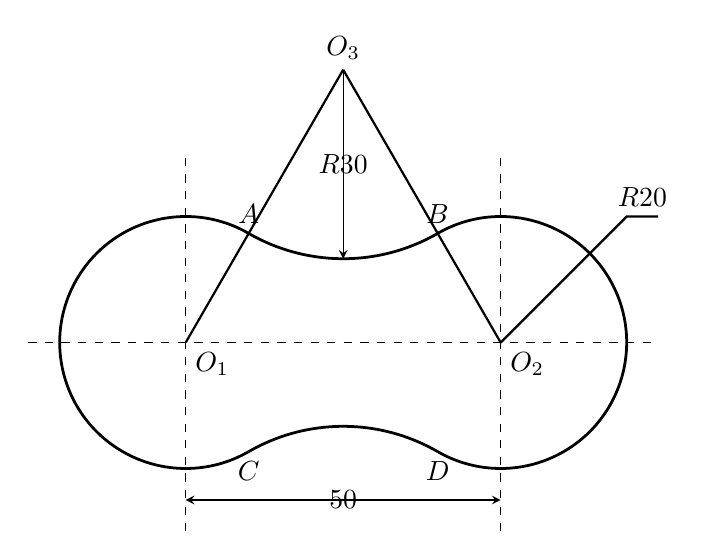
\begin{tikzpicture}[>=stealth, scale=0.8] % 箭头样式为stealth,
		
		% 绘制坐标轴
		\draw[dashed] (-5,0) -- (5,0) ; % x轴(带箭头和标签)
		\draw[dashed] (-2.5,-3) -- (-2.5,3) ; 
		\draw[dashed] (2.5,-3) -- (2.5,3) ; 
		
		\node at (2.5,0) [below right] {$O_2$};  % 原点O的标签
		\node at (-2.5,0) [below right] {$O_1$};  % 原点O的标签
		
		% 定义各关键点坐标
		% 3. 计算圆弧的起点(120°)和终点(-120°)坐标
		% 公式:圆心(x0,y0),半径r,角度θ对应的坐标为 (x0 + r·cosθ, y0 + r·sinθ)
		\coordinate (B) at (1.5, {sqrt(3)});   % 120°起点
		\coordinate (A) at (-1.5, {sqrt(3)}); % -120°终点
		\coordinate (C) at (-1.5, {-sqrt(3)});  % 点A₂
		\coordinate (D) at (1.5, {-sqrt(3)}); % 点P₂
		\coordinate (O_3) at (0,{2.5*sqrt(3)}); % 点P₂
		
		% 绘制拱形
		\draw[line width=1pt] (B) arc (120: -120:2);
		\draw[line width=1pt] (A) arc (60:300:2) ;
		
		\draw[line width=1pt] (B) arc (-60: -120:3) ;
		\draw[line width=1pt] (D) arc (60: 120:3) ;
		
		% 绘制
		\draw[thick] (2.5,0) -- (O_3) ;
		\draw[thick] (-2.5,0) -- (O_3) ;
		\draw[thick] (2.5,0) -- (4.5,2) -- (5,2) node[midway, above] {$R20$} ;
		\draw[<->] (-2.5,-2.5) -- (2.5,-2.5) node[midway] {$50$};
		\draw[->] (O_3) --++ (-90:3) node[midway] {$R30$} ;
		
		% 标记各点的标签
		\node[above] at (A) {$A$};
		\node[above] at (B) {$B$};
		\node[below] at (C) {$C$};
		\node[below] at (D) {$D$};
		\node[above] at (O_3) {$O_3$};
		
	\end{tikzpicture}
\end{document}
